\documentclass[10pt]{article}

\usepackage[T1]{fontenc}
\usepackage{newtxtext}
\usepackage{amsthm}
\usepackage{newtxmath}
\usepackage[letterpaper,top=0.72in,bottom=0.76in,left=0.78in,right=0.78in]{geometry}
\usepackage{microtype}
\usepackage{amsmath,mathtools,bm}
\usepackage{booktabs,array,tabularx,longtable,multirow}
\usepackage{enumitem}
\usepackage{graphicx}
\usepackage{caption,subcaption}
\usepackage{float}
\usepackage{xcolor}
\usepackage{tikz}
\usetikzlibrary{arrows.meta,positioning,fit,calc,shapes.geometric,decorations.pathreplacing}
\usepackage{pgfplots}
\pgfplotsset{compat=1.18}
\usepgfplotslibrary{fillbetween}
\usepackage[numbers,sort&compress]{natbib}
\usepackage{hyperref}
\usepackage[nameinlink,noabbrev]{cleveref}
\usepackage{fancyhdr}
\usepackage{lastpage}
\usepackage{titlesec}
\usepackage{eso-pic}

\definecolor{fiink}{HTML}{17232D}
\definecolor{fiblue}{HTML}{1D5F8A}
\definecolor{fiorange}{HTML}{B95F2A}
\definecolor{figreen}{HTML}{3F7356}
\definecolor{fireddark}{HTML}{8F3840}
\definecolor{figray}{HTML}{69747D}
\definecolor{fipale}{HTML}{EEF2F4}
\definecolor{fipaleorange}{HTML}{F8F1EB}
\definecolor{firule}{HTML}{D5DDE1}

\AddToShipoutPictureBG{%
  \AtPageLowerLeft{\color{white}\rule{\paperwidth}{\paperheight}}%
}

\hypersetup{
  colorlinks=true,
  linkcolor=fiblue,
  citecolor=fiblue,
  urlcolor=fiblue,
  pdftitle={The Principle of Full Invertibility},
  pdfauthor={Logan Voss},
  pdfsubject={Distinction provenance in dynamical systems and finite descriptions},
  pdfkeywords={invertibility, observability, information, distinction provenance, coarse-graining, inverse problems}
}

\setlength{\parindent}{1.15em}
\setlength{\parskip}{0.12em}
\setlength{\emergencystretch}{1em}
\setlist{nosep,leftmargin=1.5em}
\captionsetup{font=small,labelfont=bf}
\titleformat{\section}{\Large\bfseries\color{fiink}}{\thesection}{0.65em}{}
\titleformat{\subsection}{\large\bfseries\color{fiink}}{\thesubsection}{0.55em}{}
\titleformat{\subsubsection}{\normalsize\bfseries\color{fiink}}{\thesubsubsection}{0.5em}{}

\pagestyle{fancy}
\fancyhf{}
\fancyhead[L]{\small\textsc{The Principle of Full Invertibility}}
\fancyhead[R]{\small\textsc{Distinction provenance}}
\fancyfoot[C]{\small\thepage\ /\ \pageref*{LastPage}}
\renewcommand{\headrulewidth}{0.35pt}
\setlength{\headheight}{14pt}

\newtheorem{theorem}{Theorem}[section]
\newtheorem{proposition}[theorem]{Proposition}
\newtheorem{lemma}[theorem]{Lemma}
\newtheorem{corollary}[theorem]{Corollary}
\theoremstyle{definition}
\newtheorem{definition}[theorem]{Definition}
\newtheorem{principle}[theorem]{Principle}
\newtheorem{hypothesis}[theorem]{Hypothesis}
\theoremstyle{remark}
\newtheorem{remark}[theorem]{Remark}

\newcommand{\R}{\mathbb R}
\newcommand{\Torus}{\mathbb T}
\newcommand{\Zmod}{\mathbb Z}
\newcommand{\X}{\mathcal X}
\newcommand{\Y}{\mathcal Y}
\newcommand{\A}{\mathcal A}
\newcommand{\Obs}{\mathcal L}
\newcommand{\E}{\mathbb E}
\newcommand{\dt}{\Delta t}
\newcommand{\dd}{\,\mathrm d}
\newcommand{\norm}[1]{\left\lVert #1\right\rVert}
\newcommand{\abs}[1]{\left\lvert #1\right\rvert}
\newcommand{\given}{\,\middle|\,}
\newcommand{\status}[1]{\textsf{\small #1}}
\newcommand{\sourcecode}[1]{\textnormal{#1}}
\newcommand{\figsource}[1]{\par\smallskip{\footnotesize\color{figray}\textit{Source:}\enspace #1}}

\newcommand{\claimbox}[2]{%
  \begin{center}
  \fcolorbox{fiblue}{fipale}{%
    \begin{minipage}{0.94\linewidth}
    \textbf{\color{fiink}#1}\quad #2
    \end{minipage}}
  \end{center}}

\begin{document}
\pagecolor{white}

\hypersetup{pageanchor=false}
\begin{titlepage}
\thispagestyle{empty}
\vspace*{0.55in}
\noindent{\color{fiblue}\rule{\linewidth}{2.2pt}}
\vspace{0.32in}

{\fontsize{28}{33}\selectfont\bfseries\color{fiink}
The Principle of Full Invertibility\par}
\vspace{0.14in}
{\fontsize{16}{21}\selectfont\color{figray}
Distinction provenance in dynamical systems and finite descriptions\par}
\vspace{0.35in}

{\large Logan Voss\par}
\vspace{0.08in}
{\normalsize Voss Dynamics \textbar\ Working mathematical thesis and computational audit\par}
\vspace{0.05in}
{\normalsize 22 August 2026\par}

\vfill
\begin{center}
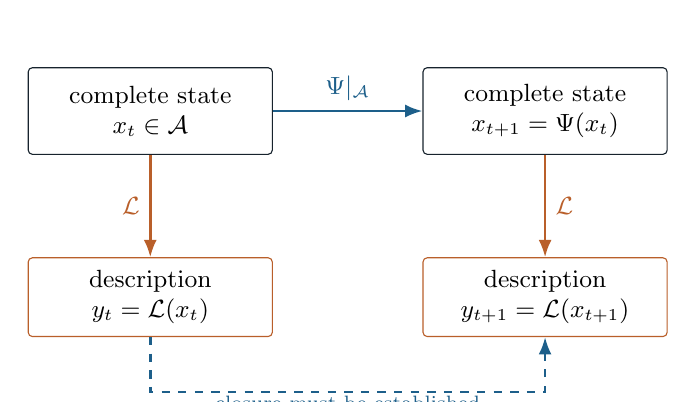
\begin{tikzpicture}[
  node distance=13mm and 19mm,
  every node/.style={font=\small,align=center},
  state/.style={draw=fiink,rounded corners=1.5pt,minimum height=11mm,minimum width=31mm,fill=white},
  desc/.style={draw=fiorange,rounded corners=1.5pt,minimum height=10mm,minimum width=31mm,fill=white},
  arrow/.style={-{Latex[length=2.2mm]},line width=0.9pt,color=fiblue},
  obs/.style={-{Latex[length=2.2mm]},line width=0.9pt,color=fiorange}
]
\node[state] (x0) {complete state\\$x_t\in\A$};
\node[state,right=of x0] (x1) {complete state\\$x_{t+1}=\Psi(x_t)$};
\node[desc,below=of x0] (y0) {description\\$y_t=\Obs(x_t)$};
\node[desc,below=of x1] (y1) {description\\$y_{t+1}=\Obs(x_{t+1})$};
\draw[arrow] (x0) -- node[above] {$\Psi|_{\A}$} (x1);
\draw[obs] (x0) -- node[left] {$\Obs$} (y0);
\draw[obs] (x1) -- node[right] {$\Obs$} (y1);
\coordinate (c0) at ([yshift=-7mm]y0.south);
\coordinate (c1) at ([yshift=-7mm]y1.south);
\draw[arrow,dashed] (y0.south) -- (c0) --
  node[below,font=\scriptsize,fill=white,inner sep=1pt]{closure must be established}
  (c1) -- (y1.south);
\end{tikzpicture}
\end{center}
\vfill

\fcolorbox{fiink}{fipale}{%
\begin{minipage}{0.94\linewidth}
\textbf{Evidence statement.}
The inverse, determinant factorization, modular criterion, phase-contraction condition, closure criterion, and fibre-cardinality results are proved under their stated assumptions. Numerical experiments locate four distinct mechanisms of apparent loss: transition folding, many-to-one observation, finite-precision access, and explicit boundary clipping. All numerical results are internal model computations; no empirical physical measurement is reported. The paper develops a mathematical audit in which each mechanism receives its own type and provenance.
\end{minipage}}

\vspace{0.35in}
\noindent{\color{fiblue}\rule{\linewidth}{0.8pt}}
\end{titlepage}
\hypersetup{pageanchor=true}

\begin{abstract}
The statement that information has been lost is incomplete until the relevant state, transition, description, inverse branch, and numerical representation are specified. This paper develops \emph{distinction provenance}: a calculus for locating the operation at which previously distinct possibilities become identical or inaccessible. A model instantiates the Principle of Full Invertibility on an admissible domain \(\A\) when its advance \(\Psi|_{\A}\) is bijective while a separate description map \(\Obs:\A\to\Y\) has nontrivial fibres.

For a drift--kick system with velocity-independent force, nonzero multiplier \(\gamma\), and coupled phases, the translational inverse is algebraic and the full smooth-stratum Jacobian factors as
\[
\det D\Psi=\gamma^{2N}\det D_\phi G_{\bm r^+}.
\]
The force Jacobian cancels from the determinant. A configuration-dependent contraction bound certifies unique phase inversion, and a finite modular analogue is bijective exactly when its velocity multiplier is a unit. An explicit three-preimage target demonstrates the complementary global phenomenon: locally nonsingular phase branches can still fold onto one future.

The same framework separates description and access from transition dynamics. In the finite phrase census, 160 complete states produce 103 descriptions, with every checked shared-description pair remaining distinct. A forensic fibre theorem characterizes when retained evidence identifies one history. Fixed-partition entropy and float64 round-trip experiments show that observational uncertainty and numerical access evolve independently of exact-state identity. Together these results turn ``where did the information go?'' into a finite audit of the core transition, boundary operation, observation map, and numerical record.
\end{abstract}

\claimbox{Primary result}{Distinguishability has provenance. Every information-loss claim should identify the complete state, the map that advanced it, the map that described it, the branch structure of the inverse, and the numerical channel through which it was retained.}

{\small\tableofcontents}
\clearpage

\section{Question, principle, and standard of proof}
\label{sec:principle}

\subsection{The question in two maps}

Let \(\X\) be a declared complete state space. Two maps play different roles:
\begin{equation}
  \Psi:\X\to\X,
  \qquad
  \Obs:\X\to\Y.
  \label{eq:two-map}
\end{equation}
\(\Psi\) advances the modeled state. \(\Obs\) records, names, bins, or summarizes it. The central discipline of this paper is to keep these maps separate. A collision under \(\Obs\) is an observational identification; a collision under \(\Psi\) is a transition identification. Neither fact determines the other.

In this study the representation map \(\Obs\) is fixed. Whether a distinction inside one fibre changes future predictions, and how the representation should be refined when it does, are separate downstream questions addressed by the later studies in the Voss Dynamics sequence.

\begin{definition}[Complete modeled state]
A state \(x\in\X\) is \emph{complete relative to the declared model} when it contains every coordinate required to evaluate one advance, while all remaining masses, frequencies, anchors, timestep choices, and control parameters are fixed and known.
\end{definition}

\begin{definition}[Distinction and provenance]
A distinction is an ordered pair \(x\neq x'\). Its \emph{provenance} is the sequence of maps through which the pair is followed. A map preserves the distinction when its two images remain unequal.
\end{definition}

\begin{definition}[Description fibre]
For \(y\in\Y\), the fibre
\begin{equation}
  \Obs^{-1}(y)
  :=
  \{x\in\X:\Obs(x)=y\}
  \label{eq:description-fibre}
\end{equation}
is the set of complete states represented by the same description.
\end{definition}

\begin{principle}[Full invertibility]
\label{principle:full-invertibility}
On an admissible domain \(\A\subseteq\X\), a model instantiates the Principle of Full Invertibility when
\begin{enumerate}
\item \(\Psi|_{\A}\) is bijective onto \(\A\);
\item \(\Obs|_{\A}\) is a separate readout and may have nontrivial fibres;
\item every claim of loss identifies whether the responsible operation is the core advance, a boundary or controller, the readout, or the finite representation.
\end{enumerate}
\end{principle}

The word \emph{full} refers to the declared state, not to universal applicability. The principle is a testable property of a specified map on a specified domain. This makes it useful even when a candidate domain contains both injective and folded regions: the same analysis locates the boundary.

\subsection{Distinction provenance}

Four map locations account for the cases studied here:
\begin{equation}
\boxed{
\begin{aligned}
\Psi_0(x)=\Psi_0(x'),\ x\neq x'
&\quad &&\text{core transition / inverse branches},\\
\mathcal B(u)=\mathcal B(u'),\ u\neq u'
&&&\text{boundary or controller collision},\\
\Obs(x)=\Obs(x'),\ x\neq x'
&&&\text{observation collision},\\
\mathcal N(r)=\mathcal N(r'),\ r\neq r'
&&&\text{finite-record collision or access limit}.
\end{aligned}}
\label{eq:provenance-taxonomy}
\end{equation}
Branch multiplicity is the inverse signature of noninjectivity in the core transition, not a separate loss mechanism. The taxonomy converts an undifferentiated statement---``information disappeared''---into four map-specific questions.

\begin{figure}[H]
\centering
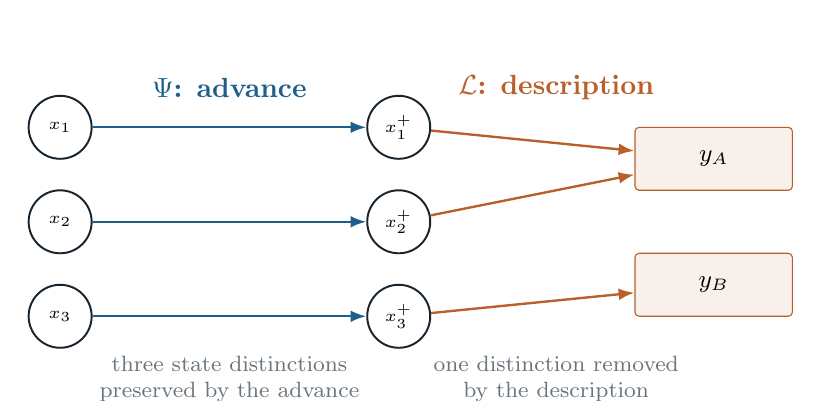
\begin{tikzpicture}[
  node distance=15mm and 24mm,
  every node/.style={font=\small,align=center},
  state/.style={circle,draw=fiink,fill=white,minimum size=8mm,line width=0.7pt},
  desc/.style={rounded corners=1.5pt,draw=fiorange,fill=fipaleorange,
               minimum width=20mm,minimum height=8mm},
  arr/.style={-{Latex[length=2mm]},line width=0.85pt,color=fiblue},
  obs/.style={-{Latex[length=2mm]},line width=0.85pt,color=fiorange}
]
\node[state] (a1) at (0,1.2) {\(\scriptstyle x_1\)};
\node[state] (a2) at (0,0) {\(\scriptstyle x_2\)};
\node[state] (a3) at (0,-1.2) {\(\scriptstyle x_3\)};
\node[state] (b1) at (4.3,1.2) {\(\scriptstyle x_1^+\)};
\node[state] (b2) at (4.3,0) {\(\scriptstyle x_2^+\)};
\node[state] (b3) at (4.3,-1.2) {\(\scriptstyle x_3^+\)};
\node[desc] (p1) at (8.3,0.8) {\(y_A\)};
\node[desc] (p2) at (8.3,-0.8) {\(y_B\)};
\draw[arr] (a1) -- (b1);
\draw[arr] (a2) -- (b2);
\draw[arr] (a3) -- (b3);
\draw[obs] (b1) -- (p1);
\draw[obs] (b2) -- (p1);
\draw[obs] (b3) -- (p2);
\node[font=\bfseries\color{fiblue}] at (2.15,1.7) {\(\Psi\): advance};
\node[font=\bfseries\color{fiorange}] at (6.3,1.7) {\(\Obs\): description};
\node[font=\footnotesize\color{figray},align=center] at (2.15,-2.0)
  {three state distinctions\\preserved by the advance};
\node[font=\footnotesize\color{figray},align=center] at (6.3,-2.0)
  {one distinction removed\\by the description};
\end{tikzpicture}
\caption{Two maps, two kinds of identity. The advance and the description are audited independently.}
\label{fig:two-map}
\end{figure}

\subsection{Claim discipline}

Three statuses are used throughout:
\begin{description}[style=nextline]
\item[\status{PROVED}] A mathematical consequence of explicitly stated assumptions.
\item[\status{COMPUTED}] An exact symbolic, enumerative, deterministic, or seeded numerical result reproduced by code, with finite-precision protocols and sample counts declared where applicable.
\item[\status{OPEN}] A theorem, domain characterization, or physical interpretation requiring further work.
\end{description}

\subsection{Contribution ledger}

\begin{table}[H]
\centering
\caption{The paper's central objects and present status.}
\label{tab:contribution-ledger}
\small
\begin{tabularx}{\linewidth}{@{}p{0.19\linewidth}X p{0.23\linewidth}@{}}
\toprule
Object & Result & Status\\
\midrule
Drift--kick inverse &
Algebraic recovery of velocity and position once a phase preimage is fixed. &
\status{PROVED}\\
Full Jacobian &
\(\det D\Psi=\gamma^{2N}\det D_\phi G_{\bm r^+}\) on smooth strata. &
\status{PROVED}\\
Phase uniqueness &
Configuration-dependent contraction certificate and exact two-clock fold criterion. &
\status{PROVED}\\
Finite analogue &
Permutation exactly when the modular multiplier is a unit. &
\status{PROVED}\\
Description fibres &
160 complete states map to 103 phrases; every checked shared-phrase pair is distinct. &
\status{COMPUTED}\\
Inverse access &
Float64 round-trip recovery quantified over contraction-certified trajectories. &
\status{COMPUTED}\\
Global admissible domain &
Characterization of a nontrivial invariant domain for the full phase-coupled map. &
\status{OPEN}\\
\bottomrule
\end{tabularx}
\end{table}

The remainder of the paper develops these objects in the order required by the audit: state and advance, inverse structure, description fibres, finite access, and applications.

\section{A structured dynamical realization}
\label{sec:model}

\subsection{State manifold}

The motivating realization contains \(N\) moving tokens and \(M\) fixed anchors. Token \(i\) carries
\begin{equation}
  z_i=(\bm r_i,\bm v_i,\theta_i,\phi_i),
  \qquad
  \bm r_i,\bm v_i\in\R^2,
  \quad
  \theta_i,\phi_i\in\Torus:=\R/(2\pi\Zmod).
  \label{eq:token-state}
\end{equation}
Here \(\bm r_i\) and \(\bm v_i\) are position and velocity, \(\theta_i\) is a directional bias, and \(\phi_i\) is an internal phase. Masses \(m_i\), intrinsic frequencies \(\omega_i\), timestep \(\dt\), anchor data, and force parameters are fixed and known. The dynamical state is
\begin{equation}
  x=(\bm r,\bm v,\bm\theta,\bm\phi)
  \in
  \X_N
  :=
  (\R^2\times\R^2\times\Torus\times\Torus)^N.
  \label{eq:state-space}
\end{equation}

Each anchor \(a\) has position \(\bm p_a\), positive weight \(Q_a\), and preferred angles \((\theta_a,\phi_a)\). Anchors are parameters of the one-step map. Any protocol that changes them defines an enlarged or externally controlled system and is treated separately.

\begin{figure}[H]
\centering
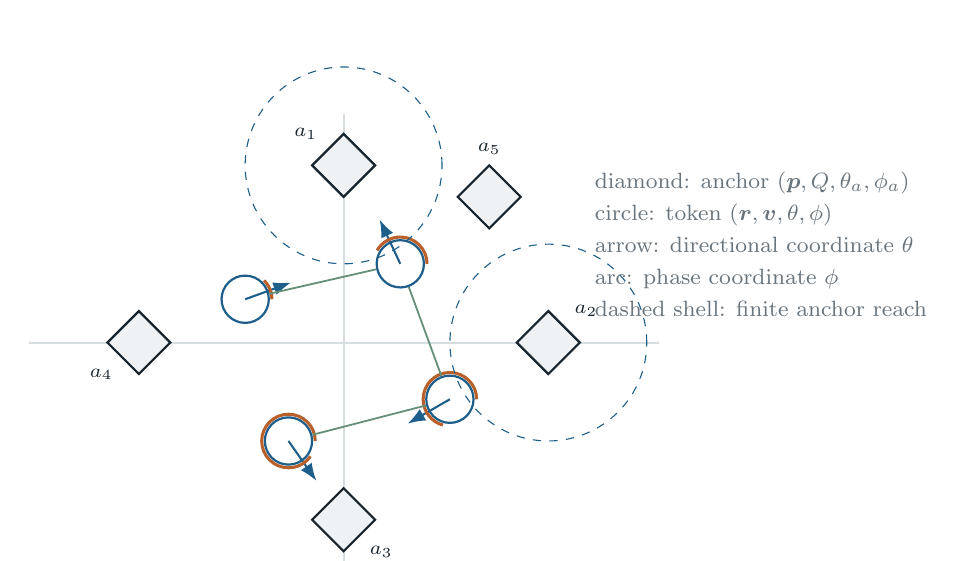
\begin{tikzpicture}[
  anchorNode/.style={regular polygon,regular polygon sides=4,rotate=45,
    draw=fiink,fill=fipale,minimum size=8mm,line width=0.8pt},
  token/.style={circle,draw=fiblue,fill=white,minimum size=6mm,line width=0.8pt},
  >=Latex
]
\draw[firule,line width=0.7pt] (-4.0,0) -- (4.0,0);
\draw[firule,line width=0.7pt] (0,-2.9) -- (0,2.9);
\node[anchorNode,label={[fiink]above:{\scriptsize \(a_1\)}}] (n) at (0,2.25) {};
\node[anchorNode,label={[fiink]right:{\scriptsize \(a_2\)}}] (e) at (2.6,0) {};
\node[anchorNode,label={[fiink]below:{\scriptsize \(a_3\)}}] (s) at (0,-2.25) {};
\node[anchorNode,label={[fiink]left:{\scriptsize \(a_4\)}}] (w) at (-2.6,0) {};
\node[anchorNode,label={[fiink]above right:{\scriptsize \(a_5\)}}] (ne) at (1.85,1.85) {};

\node[token] (t1) at (-1.25,0.55) {};
\draw[->,fiblue,line width=0.75pt] (t1.center) -- ++(20:0.62);
\draw[fiorange,line width=1.1pt] (-1.25,0.55) ++(0.34,0)
  arc[start angle=0,end angle=45,radius=0.34];
\node[token] (t2) at (0.72,1.0) {};
\draw[->,fiblue,line width=0.75pt] (t2.center) -- ++(115:0.62);
\draw[fiorange,line width=1.1pt] (0.72,1.0) ++(0.34,0)
  arc[start angle=0,end angle=150,radius=0.34];
\node[token] (t3) at (1.35,-0.72) {};
\draw[->,fiblue,line width=0.75pt] (t3.center) -- ++(210:0.62);
\draw[fiorange,line width=1.1pt] (1.35,-0.72) ++(0.34,0)
  arc[start angle=0,end angle=255,radius=0.34];
\node[token] (t4) at (-0.7,-1.25) {};
\draw[->,fiblue,line width=0.75pt] (t4.center) -- ++(305:0.62);
\draw[fiorange,line width=1.1pt] (-0.7,-1.25) ++(0.34,0)
  arc[start angle=0,end angle=325,radius=0.34];

\draw[fiblue,dashed] (n) circle[radius=1.25];
\draw[fiblue,dashed] (e) circle[radius=1.25];
\draw[figreen!80,line width=0.65pt] (t1) -- (t2) -- (t3) -- (t4) -- cycle;

\node[align=left,font=\footnotesize,text=figray] at (5.3,1.25)
  {diamond: anchor \((\bm p,Q,\theta_a,\phi_a)\)\\[2pt]
   circle: token \((\bm r,\bm v,\theta,\phi)\)\\[2pt]
   arrow: directional coordinate \(\theta\)\\[2pt]
   arc: phase coordinate \(\phi\)\\[2pt]
   dashed shell: finite anchor reach};
\end{tikzpicture}
\caption{A structured field realization. Translational, directional, and phase coordinates coexist in one declared state.}
\label{fig:field}
\end{figure}

\subsection{Ordered advance}

The practical discrete realization is a drift, a force kick, and a phase update:
\begin{subequations}
\label{eq:advance}
\begin{align}
\bm r_i^+
  &=\bm r_i+\bm v_i\dt,
  \label{eq:drift}\\
\bm v_i^+
  &=\gamma\bm v_i
  +\frac{\dt}{m_i}
  \bm F_i(\bm r^+,\bm\theta,\bm\phi),
  \label{eq:kick}\\
\phi_i^+
  &=
  \left[
  \phi_i+\omega_i\dt
  +\beta\dt\sum_{j\neq i}
  \frac{\sin(\phi_j-\phi_i)}
       {\norm{\bm r_i^+-\bm r_j^+}+\varepsilon}
  \right]_{2\pi},
  \label{eq:phase}\\
\theta_i^+&=\theta_i.
\end{align}
\end{subequations}
The structural fact is the update order. The force is evaluated at the advanced position and old angles, and it does not depend on velocity. This triangular ordering controls both the inverse and the determinant.

The force inventory is
\begin{equation}
  \bm F_i
  =
  \bm F_i^{\rm anchor}
  +\bm F_i^{\rm wave}
  +\bm F_i^{\rm pair}
  +\bm F_i^{\rm control}.
  \label{eq:force-inventory}
\end{equation}
The first term supplies finite-range directional bias, the second is a softened phase-bearing radial field, and the third combines short repulsion with intermediate attraction. A fixed external control field can be included without changing the translational inverse. The exact implementation is recorded in \cref{app:model-specification}; the inverse theorems require only velocity independence and fixed known parameters.

\subsection{Phase map}

At a known advanced position \(\bm r^+\), define
\begin{equation}
  G_{\bm r^+}(\bm\phi)
  :=
  \left[
  \bm\phi+\bm\omega\dt
  +\beta\dt\,\bm K(\bm\phi;\bm r^+)
  \right]_{2\pi},
  \label{eq:phase-map}
\end{equation}
where
\begin{equation}
  K_i(\bm\phi;\bm r^+)
  =
  \sum_{j\neq i}
  \frac{\sin(\phi_j-\phi_i)}
       {\norm{\bm r_i^+-\bm r_j^+}+\varepsilon}.
  \label{eq:phase-coupling}
\end{equation}
The full advance is therefore the composition of an explicitly invertible mechanical block and an implicit phase block. This decomposition makes the source of every inverse branch visible.

\subsection{Core and variants}

Three operations are kept distinct:
\begin{description}
\item[Core advance:] \cref{eq:advance} with no clipping and fixed parameters.
\item[Boundary variant:] an added wall rule, whose injectivity depends on how overshoot is represented.
\item[Feedback variant:] a description-dependent controller, which becomes part of the complete state if it affects future dynamics.
\end{description}
The main theorems concern the core advance. Boundary and feedback operations are valuable because they show how additional maps alter distinction provenance.

\section{Exact inverse structure}
\label{sec:inverse}

\subsection{Triangular inverse}

\begin{theorem}[Conditional exact inverse]
\label{thm:inverse}
Fix a wall-free one-step advance \cref{eq:advance}. If \(\gamma\neq0\) and the phase map \(G_{\bm r^+}\) is bijective at the advanced position, then the complete pre-state is uniquely recovered by
\begin{subequations}
\label{eq:inverse}
\begin{align}
\bm\phi
  &=G_{\bm r^+}^{-1}(\bm\phi^+),
  \label{eq:inverse-phase}\\
\bm v
  &=\gamma^{-1}
  \left[
  \bm v^+
  -\dt M^{-1}
  \bm F(\bm r^+,\bm\theta,\bm\phi)
  \right],
  \label{eq:inverse-velocity}\\
\bm r
  &=\bm r^+-\bm v\dt,
  \label{eq:inverse-position}\\
\bm\theta&=\bm\theta^+.
\end{align}
\end{subequations}
\end{theorem}

\begin{proof}
The final position is known. Bijectivity of \(G_{\bm r^+}\) determines the old phase. The force is then known because it depends on \((\bm r^+,\bm\theta,\bm\phi)\) and fixed parameters, but not on old velocity. Since \(\gamma\neq0\), \cref{eq:inverse-velocity} determines velocity; the drift then determines position. Direct substitution verifies both compositions.
\end{proof}

\begin{figure}[H]
\centering
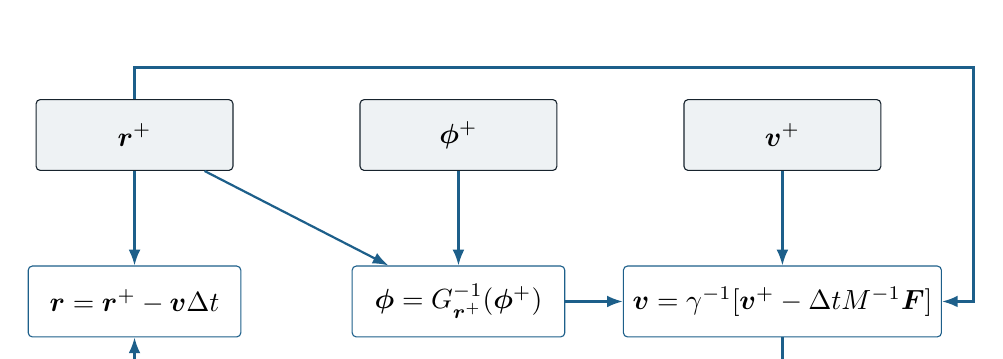
\begin{tikzpicture}[
  box/.style={rounded corners=1.5pt,draw=fiink,fill=fipale,
              minimum width=25mm,minimum height=9mm,align=center},
  known/.style={rounded corners=1.5pt,draw=fiblue,fill=white,
                minimum width=27mm,minimum height=9mm,align=center},
  arr/.style={-{Latex[length=2mm]},line width=0.8pt,color=fiblue},
  node distance=12mm and 16mm
]
\node[box] (rn) {\(\bm r^+\)};
\node[box,right=of rn] (pn) {\(\bm\phi^+\)};
\node[box,right=of pn] (vn) {\(\bm v^+\)};
\node[known,below=of pn] (po) {\(\bm\phi=G_{\bm r^+}^{-1}(\bm\phi^+)\)};
\node[known,below=of vn] (vo) {\(\bm v=\gamma^{-1}[\bm v^+-\dt M^{-1}\bm F]\)};
\node[known,below=of rn] (ro) {\(\bm r=\bm r^+-\bm v\dt\)};
\draw[arr] (rn) -- (po);
\draw[arr] (pn) -- (po);
\draw[arr] (po) -- (vo);
\coordinate (voRoute) at ([xshift=4mm]vo.east);
\coordinate (rnRoute) at ([yshift=4mm]rn.north);
\draw[arr] (rn.north) -- (rnRoute) -- (voRoute |- rnRoute) -- (voRoute) -- (vo.east);
\draw[arr] (vn) -- (vo);
\coordinate (voBottomRoute) at ([yshift=-4mm]vo.south);
\coordinate (roBottomRoute) at ([yshift=-4mm]ro.south);
\draw[arr] (vo.south) -- (voBottomRoute) -- (roBottomRoute) -- (ro.south);
\draw[arr] (rn) -- (ro);
\end{tikzpicture}
\caption{The inverse is triangular: phase branch first, then force and velocity, then position.}
\label{fig:inverse-dag}
\end{figure}

The mechanical sector is therefore globally algebraic for every velocity-independent force when \(\gamma\neq0\). All branch structure enters through the phase map.

\subsection{Full determinant factorization}

\begin{theorem}[Full Jacobian]
\label{thm:determinant}
At every smooth point of the wall-free map with static \(\bm\theta\),
\begin{equation}
\boxed{
\det D\Psi
=
\gamma^{2N}
\det D_{\bm\phi}G_{\bm r^+}(\bm\phi).
}
\label{eq:determinant}
\end{equation}
The determinant is independent of positional and phase derivatives of the force.
\end{theorem}

\begin{proof}
First change coordinates from \((\bm r,\bm v,\bm\phi)\) to
\((\bm r^+=\bm r+\dt\bm v,\bm v,\bm\phi)\); this block-triangular map has determinant one. In these coordinates, the remaining Jacobian is
\[
\begin{pmatrix}
I & 0 & 0\\
\ast & \gamma I & \dt M^{-1}D_\phi\bm F\\
\ast & 0 & D_\phi G_{\bm r^+}
\end{pmatrix}.
\]
Multiplying the diagonal block determinants yields \cref{eq:determinant}.
\end{proof}

\begin{corollary}[Local singularity channels]
The smooth full map is locally invertible exactly where
\[
\gamma\neq0
\qquad\text{and}\qquad
\det D_\phi G_{\bm r^+}\neq0.
\]
Force curvature cannot create a local singularity in this update ordering.
\end{corollary}

\begin{figure}[H]
\centering
\begin{tikzpicture}
\begin{axis}[
  width=0.68\linewidth,
  height=0.45\linewidth,
  xlabel={factorized prediction
    \(\gamma^{2N}\det D_{\phi}G_{\bm r^+}\)},
  ylabel={finite-difference \(\det D\Psi\)},
  xmin=0.18,xmax=1.0,
  ymin=0.18,ymax=1.0,
  axis lines=left,
  grid=both,
  major grid style={draw=firule},
  minor grid style={draw=firule!45},
  tick label style={font=\footnotesize},
  label style={font=\small},
  legend style={draw=none,fill=none,font=\footnotesize,at={(0.03,0.97)},anchor=north west}
]
\addplot[domain=0.18:1.0,figray,dashed,line width=0.8pt] {x};
\addlegendentry{identity line}
\addplot[
  only marks,
  mark=*,
  mark size=2.1pt,
  fiblue
] table[
  x=det_factorized,
  y=det_full,
  col sep=comma
] {evidence/determinant_factorization.csv};
\addlegendentry{15 live-map probes}
\end{axis}
\end{tikzpicture}
\caption{Numerical audit of \cref{eq:determinant}. Maximum relative discrepancy is \(2.1\times10^{-8}\).}
\label{fig:determinant}
\figsource{\sourcecode{evidence/thesis\_verification.json}, \sourcecode{determinant\_factorization}.}
\end{figure}

\subsection{Phase uniqueness}

The phase Jacobian is
\begin{equation}
\begin{aligned}
(D_\phi G)_{ii}
&=
1-\beta\dt
\sum_{j\neq i}
\frac{\cos(\phi_j-\phi_i)}
     {\widetilde d_{ij}^{+}},\\
(D_\phi G)_{ij}
&=
\beta\dt
\frac{\cos(\phi_j-\phi_i)}
     {\widetilde d_{ij}^{+}},
\qquad i\neq j,
\end{aligned}
\label{eq:phase-jacobian}
\end{equation}
where
\(\widetilde d_{ij}^{+}=\norm{\bm r_i^+-\bm r_j^+}+\varepsilon\).

\begin{theorem}[Configuration-dependent contraction certificate]
\label{thm:phase-certificate}
Define
\begin{equation}
q(\bm r^+)
:=
2\abs{\beta}\dt
\max_i\sum_{j\neq i}
\frac{1}{\widetilde d_{ij}^{+}}.
\label{eq:q}
\end{equation}
If \(q(\bm r^+)<1\), then the inverse phase iteration is a contraction in the \(\ell_\infty\) norm on a consistent torus lift. The phase preimage is unique in that lift, fixed-point inversion converges geometrically, and \(G_{\bm r^+}\) has lower bi-Lipschitz bound \(1-q\).
\end{theorem}

The certificate is configuration-dependent. It supplies an operational gate for every trajectory used in the round-trip study.

\subsection{Global branch geometry}

For two tokens at fixed softened separation \(D\), let
\[
\delta=\phi_1-\phi_2,
\qquad
\Delta\omega=\omega_1-\omega_2,
\qquad
a=\frac{2\beta\dt}{D}.
\]
The exact relative-phase map is
\begin{equation}
\boxed{
\delta^+
=
\delta+\Delta\omega\,\dt-a\sin\delta
\pmod{2\pi}.
}
\label{eq:two-clock}
\end{equation}
For equal frequencies, its derivative is \(1-a\cos\delta\). The circle map is a diffeomorphism for \(\abs a<1\), a singular monotone homeomorphism at \(\abs a=1\), and noninjective for \(\abs a>1\).

\begin{figure}[H]
\centering
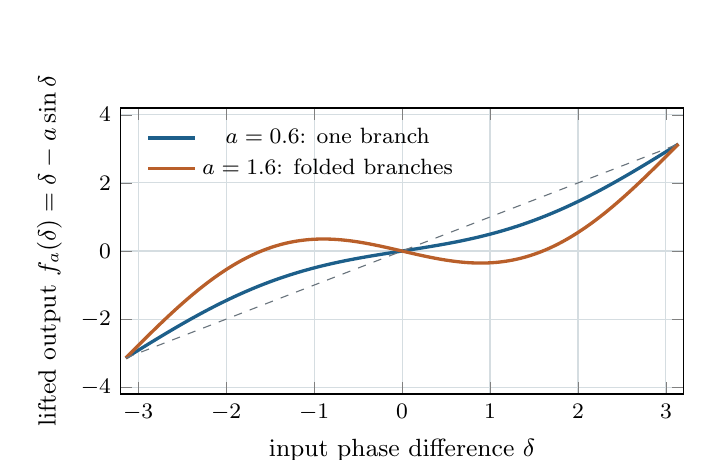
\begin{tikzpicture}
\begin{axis}[
  width=0.72\linewidth,
  height=0.43\linewidth,
  xlabel={input phase difference \(\delta\)},
  ylabel={lifted output \(f_a(\delta)=\delta-a\sin\delta\)},
  xmin=-3.2,xmax=3.2,
  ymin=-4.2,ymax=4.2,
  grid=major,
  major grid style={draw=firule},
  tick label style={font=\footnotesize},
  label style={font=\small},
  legend style={draw=none,fill=none,font=\footnotesize,at={(0.03,0.97)},anchor=north west}
]
\addplot[fiblue,line width=1.2pt,domain=-3.1416:3.1416,samples=180]
  {x-0.6*sin(deg(x))};
\addlegendentry{\(a=0.6\): one branch}
\addplot[fiorange,line width=1.2pt,domain=-3.1416:3.1416,samples=180]
  {x-1.6*sin(deg(x))};
\addlegendentry{\(a=1.6\): folded branches}
\addplot[figray,dashed,domain=-3.1416:3.1416] {x};
\end{axis}
\end{tikzpicture}
\caption{The same phase law contains an injective regime and a folded regime. Distinction provenance locates the transition between them.}
\label{fig:phase-fold}
\end{figure}

The live eight-token system reaches the folded regime at default parameters. At seed 22, step 9, one target has \(q=1.338984\) and three refined phase roots. Combining each root with the algebraic mechanical inverse produces three complete pre-states.

\begin{table}[H]
\centering
\caption{Three complete pre-states for one target. Every phase Jacobian is locally nonsingular; the distinction is global branch structure.}
\label{tab:multiroot}
\small
\begin{tabular}{@{}rrrr@{}}
\toprule
root & \(\det D_\phi G\) &
distance from generating pre-state &
forward residual\\
\midrule
0 & \(-0.2300\) & \(1.09\times10^{-15}\) & \(0\)\\
1 & \( 0.4584\) & \(7.386\) & \(1.50\times10^{-13}\)\\
2 & \( 0.4115\) & \(6.738\) & \(1.33\times10^{-13}\)\\
\bottomrule
\end{tabular}
\figsource{\sourcecode{evidence/thesis\_verification.json}, \sourcecode{phase\_multiroot\_collision}.}
\end{table}

This example demonstrates the value of the framework: a nonzero local Jacobian, a convergent inverse solver, and global branch uniqueness are separate questions.

\subsection{Finite analogue}

On \(\Zmod/M\Zmod\), consider
\begin{equation}
r^+=r+v\pmod M,
\qquad
v^+=g\,v+F(r^+)\pmod M.
\label{eq:finite-map}
\end{equation}

\begin{theorem}[Modular unit criterion]
\label{thm:finite}
\Cref{eq:finite-map} is a permutation of the \(M^2\) states for every force \(F\) if and only if \(\gcd(g,M)=1\).
\end{theorem}

\begin{proof}
If \(g\) is a unit,
\[
v=g^{-1}[v^+-F(r^+)]\pmod M,
\qquad
r=r^+-v\pmod M.
\]
If \(g\) is not a unit, multiplication by \(g\) has a nontrivial kernel, and compensated position--velocity pairs collide.
\end{proof}

Enumeration gives \(63{,}001/63{,}001\) images for \((M,g)=(251,3)\), while \((M,g)=(16,2)\) yields \(128/256\) images. The theorem provides a complete finite model of the distinction between invertible multiplication and state aggregation.

\begin{remark}[Six independent properties]
Bijectivity, local nonsingularity, time-reversal symmetry, volume preservation, energy conservation, and stable numerical inversion are distinct properties. The results above identify exactly which of them follow from each assumption.
\end{remark}

\section{Description fibres and predictive closure}
\label{sec:description}

\subsection{A finite phrase readout}

The implemented readout groups tokens by nearby anchors or marks them \texttt{FREE}. Let \(C(x)\) be this deterministic clustering and let \(P(C(x))\) be the resulting phrase. The observation map is
\begin{equation}
\Obs(x):=P(C(x)).
\label{eq:phrase-map}
\end{equation}
It retains cluster labels and counts while omitting velocities, directional coordinates, phases, exact positions, and within-cluster identity. An auxiliary geometric score,
\begin{equation}
S_{\rm geom}(x)
=
S_{\rm name}(C(x))
+S_{\rm resid}(x\mid C(x)),
\label{eq:geometric-score}
\end{equation}
summarizes phrase complexity and positional residual. The score is not needed for the fibre result; the many-to-one structure follows directly from \cref{eq:phrase-map}.

Across 160 independently evolved 14-token states,
\begin{equation}
160\ \text{complete states}
\quad\xrightarrow{\ \Obs\ }\quad
103\ \text{phrases}.
\label{eq:phrase-census}
\end{equation}
Thirty-one phrases occur more than once. Every one of 68 checked shared-phrase pairs is a pair of distinct complete states, and the largest computed fibre contains eight states.

\begin{figure}[H]
\centering
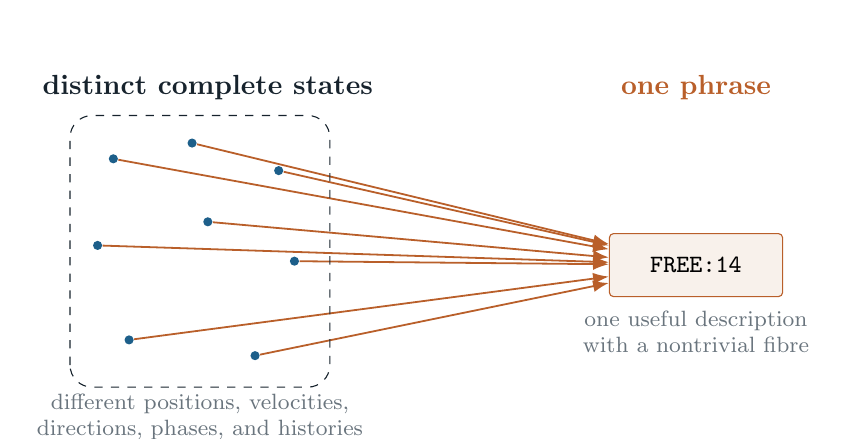
\begin{tikzpicture}[
  micro/.style={circle,fill=fiblue,minimum size=3.3pt,inner sep=0pt},
  phrase/.style={rounded corners=1.5pt,draw=fiorange,fill=fipaleorange,
                 minimum width=22mm,minimum height=8mm,font=\small\bfseries},
  obs/.style={-{Latex[length=2mm]},color=fiorange,line width=0.65pt}
]
\node[font=\bfseries\color{fiink}] at (-3.0,2.25)
  {distinct complete states};
\node[font=\bfseries\color{fiorange}] at (3.2,2.25)
  {one phrase};
\node[phrase] (p) at (3.2,0) {\texttt{FREE:14}};
\foreach \x/\y/\k in {
  -4.2/1.35/1,-3.2/1.55/2,-2.1/1.20/3,-4.4/0.25/4,
  -3.0/0.55/5,-1.9/0.05/6,-4.0/-0.95/7,-2.4/-1.15/8
} {
  \node[micro] (m\k) at (\x,\y) {};
  \draw[obs] (m\k) -- (p);
}
\draw[fiink,dashed,rounded corners=8pt]
  (-4.75,-1.55) rectangle (-1.45,1.9);
\node[font=\footnotesize,text=figray,align=center] at (-3.1,-1.93)
  {different positions, velocities,\\directions, phases, and histories};
\node[font=\footnotesize,text=figray,align=center] at (3.2,-0.85)
  {one useful description\\with a nontrivial fibre};
\end{tikzpicture}
\caption{A computed observation fibre containing eight distinct complete states.}
\label{fig:phrase-fibre}
\figsource{\sourcecode{results/battery.json}, \sourcecode{mdl\_many\_to\_one}.}
\end{figure}

\subsection{History fibres}

Let \(y=\Obs(x_t)\) be retained final evidence and suppose \(\Psi|_{\A}\) is bijective. The \(k\)-step histories compatible with \(y\) are
\begin{equation}
\mathcal H_k(y)
:=
\left\{
\Psi^{-k}(x):
x\in\Obs^{-1}(y)\cap\A
\right\}.
\label{eq:history-fibre}
\end{equation}

\begin{theorem}[Forensic fibre theorem]
\label{thm:forensic}
If \(\Psi|_{\A}\) is bijective, then
\begin{equation}
\abs{\mathcal H_k(y)}
=
\abs{\Obs^{-1}(y)\cap\A}.
\label{eq:fibre-cardinality}
\end{equation}
Consequently, retained evidence identifies one \(k\)-step history exactly when its reachable observation fibre contains one complete state.
\end{theorem}

\begin{proof}
The restriction of \(\Psi^{-k}\) to any subset of \(\A\) is a bijection onto its image and therefore preserves cardinality.
\end{proof}

The theorem separates a unique underlying predecessor from a uniquely inferable predecessor. Inverse dynamics transports the ambiguity already present in the evidence; it does not remove it.

\subsection{Description-level closure}

A many-to-one readout does not automatically define an autonomous macro-dynamics. The additional requirement is fibre compatibility, the set-level form of exact lumpability or semiconjugacy \citep{lind1995,horstmeyer2016}.

\begin{proposition}[Closure criterion]
\label{prop:closure}
Let \(\Obs:\X\to\Y\) be surjective. A deterministic map \(T:\Y\to\Y\) satisfying
\begin{equation}
T\circ\Obs=\Obs\circ\Psi
\label{eq:closure}
\end{equation}
exists if and only if
\begin{equation}
\Obs(x)=\Obs(x')
\quad\Longrightarrow\quad
\Obs(\Psi x)=\Obs(\Psi x').
\label{eq:fibre-compatibility}
\end{equation}
\end{proposition}

\begin{proof}
If \(T\) exists, \cref{eq:fibre-compatibility} follows immediately. Conversely, define \(T(y)=\Obs(\Psi x)\) for any \(x\in\Obs^{-1}(y)\); fibre compatibility makes the value independent of the chosen representative.
\end{proof}

If fibre compatibility holds for both \(\Psi\) and \(\Psi^{-1}\), the induced macro-map can itself be bijective. If it fails, the reduced process requires hidden coordinates, memory, or stochastic closure, as in projection-operator methods \citep{zwanzig1961,mori1965,chorin2000}. This is the precise bridge from description fibres to effective dynamics.

\subsection{Records and temporal order}

Complete-state retrodictability and record order are separate structures. A bijective transition pairs adjacent complete states in both directions. A recorder, by contrast, selects and stores a sequence
\[
y_t=\Obs(x_t),\qquad
y_{t+1}=\Obs(x_{t+1}),\ldots
\]
whose fibres may be nontrivial. Directional records can therefore coexist with distinction-preserving state evolution. Whether those records support a Markovian, reversible, or history-dependent macro-law is decided by \cref{prop:closure}, not by the cardinality of a single fibre alone.

\section{Information and finite access}
\label{sec:information}

\subsection{Distinctions, probability, and volume}

For a finite set \(S\subset\X\), define its distinction information by
\[
I_{\rm dist}(S):=\log_2\abs S.
\]
Every injective map preserves \(I_{\rm dist}\) on finite subsets. This is the invariant used by the principle: distinct complete alternatives remain distinct.

\begin{theorem}[Discrete entropy under a bijection]
\label{thm:shannon}
If \(X\) is a finite random state and \(Y=f(X)\) for a bijection \(f\), then
\[
H(Y)=H(X)
\]
for every probability distribution on \(X\).
\end{theorem}

\begin{proof}
The output probabilities are a permutation of the input probabilities.
\end{proof}

The finite modular experiment verifies this identity for a nonuniform distribution to \(3.6\times10^{-15}\) bits. Under the \(g=0\) many-to-one map, a uniform \(M^2\)-state distribution becomes an \(M\)-image distribution and loses exactly \(\log_2M\) bits.

Continuous differential entropy obeys a different law. Let \(X\) have an absolutely continuous distribution, let \(\Psi\) be a \(C^1\) diffeomorphism on its support, and assume \(h(X)\) and \(\E\abs{\log\abs{\det D\Psi(X)}}\) are finite. Then
\begin{equation}
h(\Psi(X))
=
h(X)
+\E\log\abs{\det D\Psi(X)}.
\label{eq:differential-entropy}
\end{equation}
Thus a bijection may contract volume and change differential entropy while preserving every exact state distinction. Invertible dissipative maps provide established examples of this separation \citep{henon1976,hoover1996,gilbert1999,ruelle1999}.

\begin{figure}[H]
\centering
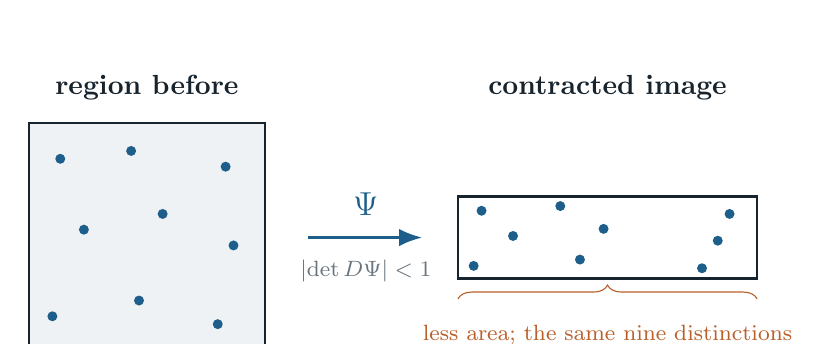
\begin{tikzpicture}[>=Latex]
\draw[fill=fipale,draw=fiink,line width=0.8pt]
  (-4,-1.45) rectangle (-1,1.45);
\node[font=\bfseries\color{fiink}] at (-2.5,1.9)
  {region before};
\foreach \x/\y in {
  -3.6/1.0,-2.7/1.1,-1.5/0.9,
  -3.3/0.1,-2.3/0.3,-1.4/-0.1,
  -3.7/-1.0,-2.6/-0.8,-1.6/-1.1
} \fill[fiblue] (\x,\y) circle (1.8pt);
\draw[->,fiblue,line width=1.2pt] (-0.45,0) -- (1.0,0);
\node[font=\large\bfseries\color{fiblue}] at (0.28,0.42) {\(\Psi\)};
\node[font=\footnotesize\color{figray}] at (0.28,-0.42)
  {\(\abs{\det D\Psi}<1\)};
\draw[fill=white,draw=fiink,line width=0.8pt]
  (1.45,-0.52) rectangle (5.25,0.52);
\node[font=\bfseries\color{fiink}] at (3.35,1.9)
  {contracted image};
\foreach \x/\y in {
  1.75/0.34,2.75/0.40,4.9/0.30,
  2.15/0.02,3.3/0.11,4.75/-0.04,
  1.65/-0.36,3.0/-0.28,4.55/-0.39
} \fill[fiblue] (\x,\y) circle (1.8pt);
\draw[decorate,decoration={brace,amplitude=5pt},fiorange]
  (1.45,-0.78) -- (5.25,-0.78);
\node[font=\footnotesize\color{fiorange},align=center] at (3.35,-1.24)
  {less area; the same nine distinctions};
\end{tikzpicture}
\caption{Volume contraction and state identification answer different questions.}
\label{fig:contraction}
\end{figure}

\subsection{A fixed observational partition}

For a quantizer \(Q:\X\to\mathcal B\), the coarse entropy \(H(Q(X_t))\) depends on the chosen partition. The corrected ensemble diagnostic declares fixed position, velocity, and circular phase bins before evolution, retains overflow bins, and reports the sum of one-dimensional marginal entropies.

\begin{figure}[H]
\centering
\begin{subfigure}[t]{0.48\linewidth}
\centering
\begin{tikzpicture}
\begin{axis}[
  width=\linewidth,height=0.68\linewidth,
  title={\(\gamma=1\)},
  xlabel={steps},ylabel={marginal entropy sum (bits)},
  xmin=0,xmax=150,ymin=0,ymax=125,
  grid=major,major grid style={draw=firule},
  tick label style={font=\scriptsize},
  label style={font=\footnotesize},
  title style={font=\small\bfseries\color{fiink}},
  legend style={draw=none,fill=none,font=\scriptsize,at={(0.98,0.98)},anchor=north east}
]
\addplot[fiblue,line width=1.1pt,mark=*]
  table[x=t,y=full_gamma1_bits,col sep=comma]
  {evidence/quantized_entropy.csv};
\addlegendentry{all coordinates}
\addplot[fiorange,line width=1.1pt,mark=square*]
  table[x=t,y=position_gamma1_bits,col sep=comma]
  {evidence/quantized_entropy.csv};
\addlegendentry{positions}
\end{axis}
\end{tikzpicture}
\end{subfigure}
\hfill
\begin{subfigure}[t]{0.48\linewidth}
\centering
\begin{tikzpicture}
\begin{axis}[
  width=\linewidth,height=0.68\linewidth,
  title={\(\gamma=0.982\)},
  xlabel={steps},ylabel={marginal entropy sum (bits)},
  xmin=0,xmax=150,ymin=0,ymax=125,
  grid=major,major grid style={draw=firule},
  tick label style={font=\scriptsize},
  label style={font=\footnotesize},
  title style={font=\small\bfseries\color{fiink}},
  legend style={draw=none,fill=none,font=\scriptsize,at={(0.98,0.98)},anchor=north east}
]
\addplot[fiblue,line width=1.1pt,mark=*]
  table[x=t,y=full_gamma0982_bits,col sep=comma]
  {evidence/quantized_entropy.csv};
\addlegendentry{all coordinates}
\addplot[fiorange,line width=1.1pt,mark=square*]
  table[x=t,y=position_gamma0982_bits,col sep=comma]
  {evidence/quantized_entropy.csv};
\addlegendentry{positions}
\end{axis}
\end{tikzpicture}
\end{subfigure}
\caption{A fixed observer partition evolves differently from exact distinction cardinality. The plotted quantity is a sum of marginals, not a joint state entropy.}
\label{fig:fixed-entropy}
\figsource{\sourcecode{evidence/thesis\_verification.json}, \texttt{fixed\_partition\_marginal\_entropy}.}
\end{figure}

The \(\gamma=1\) full marginal sum rises from \(84.62\) to \(110.40\) bits by \(t=150\). For \(\gamma=0.982\), it rises to \(103.31\) bits at \(t=30\) and settles at \(99.26\) bits by \(t=150\). These values describe the observer's fixed alphabet. They do not count exact-state collisions.

\subsection{A state is not a snapshot}

Projection onto position,
\[
\pi_r(x)=\bm r,
\]
removes velocity and phase coordinates required by the inverse. In a 10-token, 30-step probe, the complete final state returns to its origin with \(L^2=1.31\times10^{-10}\). Zeroing final velocities first gives \(L^2=15.35\); zeroing phases gives \(25.37\). The scale separation directly demonstrates state sufficiency: a visible configuration and a complete dynamical state are different objects.

\subsection{Float64 round-trip access}

On a trajectory for which every phase update satisfies \(q<1\), the exact branch is unique. Finite arithmetic introduces a second question: how accurately can that branch be recovered from the stored endpoint? Linearization gives the schematic amplification
\begin{equation}
\norm{\delta x_{t-T}}
\lesssim
\left(
\prod_{s=0}^{T-1}
\norm{D\Psi^{-1}(x_{t-s})}
\right)
\norm{\epsilon_t}
+\text{accumulated roundoff}.
\label{eq:error-amplification}
\end{equation}

\begin{figure}[t]
\centering
\begin{tikzpicture}
\begin{axis}[
  width=0.84\linewidth,
  height=0.47\linewidth,
  xlabel={forward steps before endpoint inversion},
  ylabel={\(\log_{10} L^2\) round-trip error},
  xmin=35,xmax=205,
  ymin=-14.2,ymax=4.8,
  grid=both,
  major grid style={draw=firule},
  minor grid style={draw=firule!45},
  tick label style={font=\footnotesize},
  label style={font=\small},
  legend style={draw=none,fill=none,font=\footnotesize,
                at={(0.02,0.97)},anchor=north west}
]
\addplot[draw=none,name path=g1low,forget plot]
  table[x=steps,y=p10_log10_l2,col sep=comma]
  {evidence/information_horizon_gamma1.csv};
\addplot[draw=none,name path=g1high,forget plot]
  table[x=steps,y=p90_log10_l2,col sep=comma]
  {evidence/information_horizon_gamma1.csv};
\addplot[fiblue!16,forget plot] fill between[of=g1low and g1high];
\addplot[fiblue,line width=1.2pt,mark=*]
  table[x=steps,y=median_log10_l2,col sep=comma]
  {evidence/information_horizon_gamma1.csv};
\addlegendentry{\(\gamma=1\), median and 10--90\% band}

\addplot[draw=none,name path=gdlow,forget plot]
  table[x=steps,y=p10_log10_l2,col sep=comma]
  {evidence/information_horizon_gamma0982.csv};
\addplot[draw=none,name path=gdhigh,forget plot]
  table[x=steps,y=p90_log10_l2,col sep=comma]
  {evidence/information_horizon_gamma0982.csv};
\addplot[fiorange!18,forget plot] fill between[of=gdlow and gdhigh];
\addplot[fiorange,line width=1.2pt,mark=square*]
  table[x=steps,y=median_log10_l2,col sep=comma]
  {evidence/information_horizon_gamma0982.csv};
\addlegendentry{\(\gamma=0.982\), median and 10--90\% band}
\addplot[figray,dashed,domain=35:205] {-6};
\end{axis}
\end{tikzpicture}
\caption{Float64 round-trip recovery on trajectories certified by \(q<1\) and a converged wrapped phase residual.}
\label{fig:roundtrip}
\figsource{\sourcecode{evidence/thesis\_verification.json}; 144 endpoint inversions before certification filters.}
\end{figure}

At \(T=200\), the certified median error is \(3.02\times10^{-6}\) for \(\gamma=1\) over 12 seeds and \(3.04\times10^{-3}\) for \(\gamma=0.982\) over 8 seeds. The damped 10--90\% range spans \(2.86\times10^{-5}\) to \(1.69\). This trajectory- and precision-dependent access scale is an \emph{epistemic horizon}: the branch may remain mathematically unique after the stored endpoint ceases to recover it at the desired tolerance.

\section{Distinction provenance in action}
\label{sec:demonstrations}

\subsection{Four located mechanisms}

The model and evidence package exhibit four distinct outcomes under one common audit.

\begin{table}[H]
\centering
\caption{Distinction provenance across the audited model.}
\label{tab:provenance}
\small
\begin{tabularx}{\linewidth}{@{}p{0.20\linewidth}p{0.25\linewidth}X@{}}
\toprule
Mechanism & Diagnostic object & Located result\\
\midrule
Transition folding &
Phase preimages of one target &
Three complete pre-states share one future; the loss occurs in the phase advance.\\
Boundary clipping &
Two in-domain overshoots &
States at distance \(0.2\) become identical under the clamp; the loss occurs at the wall operation.\\
Observation fibre &
Anchor-labelled phrase &
160 states produce 103 phrases; the loss occurs in the readout.\\
Finite access &
Endpoint inverse in float64 &
Recovery error grows with horizon on unique certified branches; the loss is practical access at a chosen tolerance.\\
\bottomrule
\end{tabularx}
\end{table}

These outcomes are not competing explanations of the same event. The core transition and an optional boundary or controller act in sequence; description and numerical storage are separate representations of the retained complete state:
\begin{equation}
\boxed{
\begin{aligned}
x&\xrightarrow{\ \Psi_0\ }u\xrightarrow{\ \mathcal B\ }x^+,
&&\text{core advance and optional boundary},\\
x^+&\xrightarrow{\ \Obs\ }y,
&&\text{description branch},\\
x^+&\xrightarrow{\ \mathcal N\ }\widehat{x}^{+},
&&\text{stored numerical-state branch}.
\end{aligned}
}
\label{eq:pipeline}
\end{equation}
Here \(\mathcal B\) may be the identity when no boundary or controller is present. The provenance question asks for the first map at which a chosen distinction is merged or becomes inaccessible.

\subsection{Boundary clipping as an exact operation}

\begin{proposition}[Wall-clamp collision]
\label{prop:wall}
Let one force-free coordinate have wall \(w\), equal velocities \(v>0\), and two in-domain positions \(r_1\neq r_2<w\) satisfying
\[
r_1+v\dt>w,
\qquad
r_2+v\dt>w.
\]
If the boundary rule replaces every overshoot by \(w\) and multiplies both velocities by the same bounce factor, the two states have one image.
\end{proposition}

\begin{proof}
The clamp sends both advanced positions to \(w\); equal velocities receive the same update; all other coordinates are equal.
\end{proof}

The computational construction uses \(w=3.6\), pre-state distance \(0.2\), and produces final distance zero. The proposition gives a precise engineering lesson: an invertible boundary must retain overshoot, for example by periodic wrapping on a torus or exact specular reflection.

\subsection{Relational phase transport}

The two-clock law \cref{eq:two-clock} also yields an exact retained relation. When coupling is switched off after step \(n_0\),
\begin{equation}
\delta_n
=
\delta_{n_0}
+(n-n_0)\Delta\omega\,\dt
\pmod{2\pi}.
\label{eq:decoupled-phase}
\end{equation}
Equivalently, the co-rotating coordinate
\[
I_n:=\delta_n-n\Delta\omega\,\dt
\]
is conserved. Equal frequencies reduce this to conservation of the raw phase difference.

\begin{figure}[H]
\centering
\begin{subfigure}[t]{0.49\linewidth}
\centering
\begin{tikzpicture}
\begin{axis}[
  width=\linewidth,height=0.69\linewidth,
  xlabel={uncoupled steps},
  ylabel={\(\abs{\delta}\) (radians)},
  xmin=0,xmax=305,ymin=0,ymax=3.1,
  grid=major,major grid style={draw=firule},
  tick label style={font=\scriptsize},
  label style={font=\footnotesize},
  legend style={draw=none,fill=none,font=\scriptsize,
                at={(0.03,0.97)},anchor=north west}
]
\addplot[fiblue,line width=1.2pt,mark=*]
  table[x=t,y=equal_delta_rad,col sep=comma]
  {evidence/clock_memory.csv};
\addlegendentry{\(\omega_1=\omega_2\)}
\addplot[fiorange,line width=1.2pt,mark=square*]
  table[x=t,y=unequal_delta_rad,col sep=comma]
  {evidence/clock_memory.csv};
\addlegendentry{\(\omega_1\neq\omega_2\)}
\end{axis}
\end{tikzpicture}
\caption{Relative phase.}
\end{subfigure}
\hfill
\begin{subfigure}[t]{0.49\linewidth}
\centering
\begin{tikzpicture}
\begin{axis}[
  width=\linewidth,height=0.69\linewidth,
  xlabel={uncoupled steps},
  ylabel={two-clock order parameter \(R\)},
  xmin=0,xmax=305,ymin=0.2,ymax=1.03,
  grid=major,major grid style={draw=firule},
  tick label style={font=\scriptsize},
  label style={font=\footnotesize},
  legend style={draw=none,fill=none,font=\scriptsize,
                at={(0.03,0.05)},anchor=south west}
]
\addplot[fiblue,line width=1.2pt,mark=*]
  table[x=t,y=equal_R,col sep=comma]
  {evidence/clock_memory.csv};
\addlegendentry{\(\omega_1=\omega_2\)}
\addplot[fiorange,line width=1.2pt,mark=square*]
  table[x=t,y=unequal_R,col sep=comma]
  {evidence/clock_memory.csv};
\addlegendentry{\(\omega_1\neq\omega_2\)}
\end{axis}
\end{tikzpicture}
\caption{Coherence.}
\end{subfigure}
\caption{After four coupling steps, \(\beta\) is set exactly to zero. Equal-frequency phase difference is retained; unequal-frequency drift follows \cref{eq:decoupled-phase} to floating-point precision.}
\label{fig:phase-transport}
\figsource{\sourcecode{evidence/thesis\_verification.json}, \texttt{decoupled\_clock\_memory\_and\_readout}.}
\end{figure}

\subsection{Controlled local response}

Resetting one phase is an intervention. Clone one phase state into a reset arm and a no-reset control, alter only the separation, and compare the partner after one step. The exact difference is
\begin{equation}
\Delta_{\rm reset}\phi_2^+
=
\frac{\beta\dt}{\widetilde D}
\left[
\sin(\phi_{1,\rm reset}-\phi_2)
-
\sin(\phi_{1,\rm control}-\phi_2)
\right].
\label{eq:reset-response}
\end{equation}
Measured effects are \(0.32266\) radians at distance \(0.3\) and \(0.004047\) radians at distance \(24\), matching the softened \(1/\widetilde D\) ratio. The partner does not change in the same instant; the next advance transmits the controlled response. This supplies a clean example of relational memory, local intervention, and distance-weighted dynamics within one exact phase law.

\subsection{What the demonstrations establish}

The multiroot, wall, phrase, and round-trip experiments form a single positive result: the framework identifies \emph{which operation} owns each loss of distinguishability. This is stronger than labeling every ambiguity ``entropy'' or every failed reconstruction ``irreversibility.'' It produces a typed result that can be carried into other dynamical, observational, and computational systems.

\section{Implications of distinction provenance}
\label{sec:implications}

\subsection{A five-question audit}

The framework reduces an information-loss claim to five questions:
\begin{enumerate}
\item What is the complete modeled state?
\item Which map advances it?
\item Which map describes or records it?
\item Is the relevant inverse branch unique?
\item Is that branch recoverable at the available precision?
\end{enumerate}
The order matters. A partial record cannot answer a question about complete-state identity until the observation fibre is characterized; a numerical inverse cannot establish uniqueness until branch structure is known.

\begin{figure}[H]
\centering
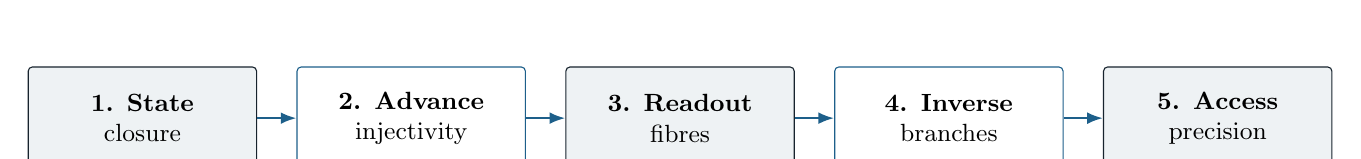
\begin{tikzpicture}[
  stage/.style={rounded corners=1.5pt,draw=fiink,fill=fipale,
                minimum width=29mm,minimum height=13mm,align=center,font=\small},
  test/.style={rounded corners=1.5pt,draw=fiblue,fill=white,
               minimum width=29mm,minimum height=13mm,align=center,font=\small},
  arr/.style={-{Latex[length=2mm]},line width=0.85pt,color=fiblue},
  node distance=5mm
]
\node[stage] (s1) {\textbf{1. State}\\closure};
\node[test,right=of s1] (s2) {\textbf{2. Advance}\\injectivity};
\node[stage,right=of s2] (s3) {\textbf{3. Readout}\\fibres};
\node[test,right=of s3] (s4) {\textbf{4. Inverse}\\branches};
\node[stage,right=of s4] (s5) {\textbf{5. Access}\\precision};
\draw[arr] (s1) -- (s2);
\draw[arr] (s2) -- (s3);
\draw[arr] (s3) -- (s4);
\draw[arr] (s4) -- (s5);
\end{tikzpicture}
\caption{The distinction-provenance audit. Each stage answers a different identity question.}
\label{fig:audit}
\end{figure}

\subsection{Dynamics and information theory}

The determinant theorem separates local volume change from state identity. This is consistent with established invertible dissipative maps \citep{henon1976,hoover1996,gilbert1999}: contraction is a geometric property of an ensemble, while injectivity is a property of point identity. The phase-fold example adds the complementary lesson that nonzero local Jacobians do not settle global branch uniqueness.

The observation map introduces a second, independent information structure. Discrete Shannon entropy is invariant under a finite permutation \citep{shannon1948a,shannon1948b,cover2006}; differential entropy changes by the expected log-Jacobian; coarse entropy depends on a partition; and description fibres determine which complete states a record can distinguish. Treating these as separate quantities gives entropy statements a precise mathematical owner.

\subsection{Causality and records}

Invertibility, time-reversal symmetry, intervention direction, thermodynamic irreversibility, and record order need not coincide. The transition map may admit a unique inverse without possessing a physical time-reversal involution. A recorder may accumulate descriptions in one order even when adjacent complete states determine one another. An autonomous macro-law exists only under the closure criterion \cref{prop:closure}.

This decomposition replaces a single overloaded word with explicit structures:
\[
\text{transition orientation},\quad
\text{retrodictive relation},\quad
\text{intervention response},\quad
\text{record order}.
\]
Each can be tested without assigning the properties of one to another.

\subsection{Forensic reconstruction}

\Cref{thm:forensic} gives a direct rule for reconstruction. If the reachable observation fibre is a singleton, the evidence identifies one complete present and therefore one history on a bijective domain. If the fibre contains several states, the scientifically correct output is the transported history family \(\mathcal H_k(y)\).

This distinction is immediately applicable to logs, simulations, market records, event traces, and physical measurements. It separates
\[
\text{one modeled past}
\qquad\text{from}\qquad
\text{one past identified by retained evidence}.
\]
The framework therefore supports both exact reconstruction and principled ambiguity reporting.

\subsection{Simulation, telemetry, and digital twins}

In software and scientific computing, the two-map architecture becomes
\[
\text{state transition}
\quad\Vert\quad
\text{telemetry summarization}.
\]
A dashboard collision is not a state collision. Conversely, a dashboard cannot reconstruct state unless its fibre is known to be a singleton on the reachable set. Systems designed for later inversion should:
\begin{enumerate}
\item retain every closure variable and controller parameter;
\item preserve intervention and boundary histories;
\item checkpoint before round-trip error exceeds the required tolerance;
\item validate recovery over ensembles rather than one trajectory;
\item report solver convergence separately from branch uniqueness.
\end{enumerate}

The float64 study turns these principles into an instrumentation objective: extend the recovery horizon by selecting state coordinates, precision, and checkpoint cadence deliberately.

\subsection{Observation design}

The fibre viewpoint gives every sensor system a measurable target. A readout is adequate for a task when its reachable fibres preserve the distinctions required by that task. This is weaker than demanding a globally injective sensor and stronger than assuming a low-error summary is sufficient.

Delay-coordinate methods provide one path from partial observation to state reconstruction \citep{takens1981,sauer1991}. The relevant question is not whether a single snapshot is complete, but whether a declared history of observations embeds the reachable state set with acceptable conditioning.

\subsection{A transferable scientific method}

The resulting workflow is
\begin{equation}
\boxed{
\text{declare}
\longrightarrow
\text{advance}
\longrightarrow
\text{observe}
\longrightarrow
\text{invert}
\longrightarrow
\text{locate}.
}
\label{eq:workflow}
\end{equation}
Declare the complete state and parameters. Advance by a specified map. Observe through an explicit readout. Invert with branch and precision diagnostics. Locate the first operation that removes or obscures the distinction of interest. This is the principal methodological contribution of the paper.

\section{Scope and open theorem program}
\label{sec:scope}

\subsection{Scope of the present results}

The paper establishes a conditional principle and a model-level audit. Its scope is defined by the following boundaries:
\begin{enumerate}
\item The translational inverse is global for \(\gamma\neq0\) and velocity-independent force; the full inverse additionally requires a unique phase branch.
\item The certificate \(q(\bm r^+)<1\) proves uniqueness for an individual phase update. A nontrivial invariant domain on which it holds for all time remains to be characterized.
\item Jacobian and differential-entropy identities apply on smooth strata. The finite anchor cutoffs are piecewise smooth.
\item The phrase readout is a deterministic geometric clustering with an auxiliary score. It is not required to be a complete code.
\item The round-trip experiment measures end-to-end float64 recovery, not an independently estimated condition number.
\item The model separates exact-state, observational, and numerical information. A thermodynamic theory would additionally require energy, reservoirs, temperature, and a physical measure.
\item The equations define a mathematical system. Applying the principle to a physical domain requires an independently justified complete state, calibrated parameters, and prospective tests.
\end{enumerate}
These boundaries delimit the theorem without reducing its generality as an audit method.

\subsection{Global phase domain}

The phase Jacobian is an identity minus a signed weighted graph Laplacian. The principal open theorem is to characterize the largest domain on which \(G_{\bm r}\) is globally bijective and invariant under the full advance. Promising routes include:
\begin{enumerate}
\item spectral bounds sharper than the \(\ell_\infty\) certificate \(q<1\);
\item degree-theoretic continuation of the torus map;
\item explicit branch-bifurcation analysis beyond the two-clock reduction;
\item invariant minimum-separation estimates for the coupled translational dynamics.
\end{enumerate}

\subsection{Invertible boundaries}

The clamp in \cref{prop:wall} can be replaced by a distinction-preserving boundary:
\begin{itemize}
\item periodic position on a two-torus;
\item exact specular reflection retaining overshoot;
\item an enlarged state that records the boundary impulse and traversed distance.
\end{itemize}
Each option yields a different but explicitly auditable state space.

\subsection{Continuous-time realization}

A smooth continuous counterpart is
\begin{subequations}
\begin{align}
\dot{\bm r}_i&=\bm v_i,\\
\dot{\bm v}_i&=-\kappa\bm v_i+m_i^{-1}\bm F_i(\bm r,\bm\theta,\bm\phi),\\
\dot\phi_i&=\omega_i+\beta\sum_{j\neq i}
\frac{\sin(\phi_j-\phi_i)}
{\norm{\bm r_i-\bm r_j}+\varepsilon}.
\end{align}
\label{eq:continuous}
\end{subequations}
For a globally Lipschitz vector field, uniqueness of solutions gives an invertible finite-time flow wherever solutions exist. Liouville's general formula,
\[
\det D\Phi_t(x_0)
=
\exp\left(
\int_0^t\nabla\cdot f(x_s)\,\dd s
\right),
\]
then relates volume contraction to the divergence without identifying trajectories. A smooth taper at the anchor cutoff would place the complete realization inside this theorem.

\subsection{Recovery bounds}

The computed round-trip curves motivate a trajectory-level error theorem. Let
\[
\kappa_T(x_t):=\norm{D\Psi^{-T}(x_t)}.
\]
A useful bound would expose the velocity multiplier, phase singular values, and force Lipschitz constants:
\begin{equation}
\norm{\widehat x_{t-T}-x_{t-T}}
\le
C_T\epsilon,
\qquad
C_T
\lesssim
\prod_{s=0}^{T-1}
\frac{c_s}
{\abs{\gamma}\,\sigma_{\min}(D_\phi G_s)}.
\label{eq:horizon-bound}
\end{equation}
Given a tolerance \(\tau\), the largest \(T\) for which \(C_T\epsilon\le\tau\) would provide a certified numerical access horizon.

\subsection{Observability from histories}

The state-sufficiency result invites a delay-coordinate analysis. For a readout \(y_t=h(x_t)\), determine when
\[
(y_t,y_{t-\tau},\ldots,y_{t-(m-1)\tau})
\]
embeds the reachable set, how large \(m\) must be, and how inverse conditioning scales with noise. This would connect exact-state theory to realistic partial instrumentation.

\subsection{Description-level dynamics}

The closure criterion \cref{prop:closure} should be evaluated directly for the phrase readout and for task-specific alternatives. When closure fails, one can quantify the memory order required for a predictive description. When it holds in both directions, the induced macro-law inherits invertibility even though the readout is many-to-one.

\subsection{Research sequence}

\[
\boxed{
\text{phase domain}
\longrightarrow
\text{invertible boundary}
\longrightarrow
\text{recovery bound}
\longrightarrow
\text{history observability}
\longrightarrow
\text{domain tests}.
}
\]
This sequence advances the principle from exact one-step structure to certified long-horizon and domain-specific use.

\section{Conclusion: the provenance of distinction}
\label{sec:conclusion}

The Principle of Full Invertibility begins with a simple separation:
\[
\Psi:\text{complete state}\longrightarrow\text{complete state},
\qquad
\Obs:\text{complete state}\longrightarrow\text{description}.
\]
From that separation follows a complete audit of distinguishability.

The drift--kick realization supplies exact mechanics. Once a phase branch is fixed, velocity and position recover algebraically. The full Jacobian factors into a velocity multiplier and a phase determinant,
\[
\det D\Psi
=
\gamma^{2N}\det D_\phi G_{\bm r^+},
\]
independently of force curvature. The phase certificate \(q<1\) identifies a unique inverse chamber for each tested update. The two-clock reduction exposes the complementary folded regime, and the three-preimage construction shows that local nonsingularity and global branch identity are distinct. The modular theorem closes the same question exactly on a finite state space.

The description layer supplies a second geometry. Its fibres collect complete states that share one retained name. The forensic fibre theorem transports those fibres backward without changing their cardinality. The closure criterion determines when a readout supports autonomous macro-dynamics. Fixed-partition entropy and float64 round trips then separate observational uncertainty from finite numerical access.

Together, these results produce a typed provenance calculus whose operations are audited separately:
\[
\boxed{
\begin{aligned}
\Psi_0 &: x\mapsto u && \text{core advance},\\
\mathcal B &: u\mapsto x^+ && \text{boundary or controller},\\
\Obs &: x^+\mapsto y && \text{description branch},\\
\mathcal N &: x^+\mapsto\widehat{x}^{+} && \text{numerical-state branch}.
\end{aligned}
}
\]
Each operation has its own injectivity or access question. Inverse branch multiplicity is the
signature of noninjectivity in the preceding transition. This is the paper's
principal contribution.

The most transferable conclusion is therefore:
\begin{quote}
\large\itshape
A state may have one past while every available description of it has many; the difference is determined by the maps through which the distinction passed.
\end{quote}

Information loss is no longer a free-standing diagnosis. It is a located event. One declares the state, advances it, observes it, resolves its inverse branches, computes numerical access, and identifies the first operation at which the distinction is merged or becomes inaccessible. That is the provenance of distinction, and it is the operational content of full invertibility.


\appendix
\section{Supplementary proofs}
\label{app:proofs}

\subsection{Mechanical block determinant}

Let \(d=2N\), \(F_r=D_{\bm r^+}\bm F\), and first take unit masses for notational clarity. From
\[
\bm r^+=\bm r+\dt\bm v,
\qquad
\bm v^+=\gamma\bm v+\dt\bm F(\bm r^+),
\]
the mechanical Jacobian is
\[
D\Psi_{rv}
:=
\begin{pmatrix}
I_d & \dt I_d\\
\dt F_r & \gamma I_d+\dt^2F_r
\end{pmatrix}.
\]
The Schur complement of \(I_d\) is \(\gamma I_d\), hence
\[
\det D\Psi_{rv}=\gamma^d=\gamma^{2N}.
\]
For diagonal mass matrix \(M\), the two terms containing
\(\dt^2M^{-1}F_r\) cancel identically.

\subsection{Phase contraction proof}

Write
\[
K_i(\bm\phi)
:=
\sum_{j\neq i}
w_{ij}\sin(\phi_j-\phi_i),
\qquad
w_{ij}
:=
(\widetilde d_{ij}^+)^{-1}.
\]
Using \(\abs{\sin u-\sin v}\le\abs{u-v}\),
\begin{align*}
\abs{K_i(\bm\phi)-K_i(\bm\psi)}
&\le
\sum_{j\neq i}w_{ij}
\abs{(\phi_j-\phi_i)-(\psi_j-\psi_i)}\\
&\le
2\left(\sum_{j\neq i}w_{ij}\right)
\norm{\bm\phi-\bm\psi}_\infty.
\end{align*}
Therefore the inverse fixed-point map has Lipschitz constant at most
\[
q(\bm r^+)
:=
2\abs{\beta}\dt
\max_i\sum_{j\neq i}w_{ij}.
\]
When \(q<1\), Banach's theorem gives a unique fixed point on the chosen lift and geometric convergence. The forward lift \(G(\phi)=\phi+h(\phi)\) obeys
\[
\norm{G(\phi)-G(\psi)}_\infty
\ge
(1-q)\norm{\phi-\psi}_\infty,
\]
which gives injectivity and the lower bi-Lipschitz bound.

\subsection{Two-clock regime}

For two clocks,
\[
\phi_1^+
:=
\phi_1+\omega_1\dt
+\frac{\beta\dt}{D}\sin(\phi_2-\phi_1),
\]
\[
\phi_2^+
:=
\phi_2+\omega_2\dt
+\frac{\beta\dt}{D}\sin(\phi_1-\phi_2).
\]
Subtracting gives \cref{eq:two-clock}. For equal frequencies,
\[
f_a(\delta)=\delta-a\sin\delta,
\qquad
f_a'(\delta)=1-a\cos\delta.
\]
If \(\abs a<1\), then \(f_a'>0\) everywhere and the degree-one circle map is a diffeomorphism. If \(\abs a=1\), the derivative is nonnegative and vanishes only at isolated points, so the map remains a strictly monotone homeomorphism but its inverse derivative is singular: at \(\delta=0\pmod{2\pi}\) for \(a=1\), and at \(\delta=\pi\pmod{2\pi}\) for \(a=-1\). If \(\abs a>1\), the derivative changes sign: for \(a>1\), \(f_a'(0)<0<f_a'(\pi)\); for \(a<-1\), \(f_a'(\pi)<0<f_a'(0)\). In either case the lift has local extrema and is noninjective.

Linearization at \(\delta=0\) gives
\[
\delta^+=(1-a)\delta+O(\delta^3).
\]
Thus synchronization is hyperbolically stable for \(0<a<2\). At \(a=2\),
\[
f_2^2(\delta)
:=
\delta-\frac23\delta^3
+\frac{11}{30}\delta^5
+O(\delta^7),
\]
so the fixed point remains locally asymptotically stable with algebraic convergence. For \(a>2\), it is unstable.

\subsection{The \(\gamma=0\) collision}

Choose \(\bm v_2\neq\bm v_1\) and
\[
\bm r_2
:=
\bm r_1-(\bm v_2-\bm v_1)\dt.
\]
Then
\[
\bm r_1+\bm v_1\dt
=
\bm r_2+\bm v_2\dt
=
\bm r^+.
\]
At \(\gamma=0\), both final velocities equal
\(\dt M^{-1}\bm F(\bm r^+,\bm\theta,\bm\phi)\); the phase updates also agree. Distinct pre-states have one image.

\subsection{Wall-clamp collision}

Take two in-domain positions \(r_1\neq r_2<w\) and equal velocity \(v>0\) such that both drifts overshoot \(w\). A clamp sends both positions to \(w\) and applies the same bounce multiplier to both velocities. Every output coordinate then agrees. This proves \cref{prop:wall}.

\subsection{Finite entropy identities}

For a permutation \(f:S\to S\),
\[
p_{f(X)}(y)=p_X(f^{-1}(y)),
\]
so the output probability list is a rearrangement of the input list and \(H(f(X))=H(X)\).

For a many-to-one map,
\[
p_Y(y)=\sum_{x\in f^{-1}(y)}p_X(x).
\]
In the uniform \(g=0\) modular system, \(M^2\) states map evenly to \(M\) images, giving
\[
H(X)=2\log_2M,
\qquad
H(Y)=\log_2M.
\]

\subsection{Differential entropy transformation}

Under the regularity and integrability assumptions stated before \cref{eq:differential-entropy},
\[
\rho_Y(y)
:=
\frac{\rho_X(x)}
{\abs{\det D\Psi(x)}},
\qquad x=\Psi^{-1}(y).
\]
Changing variables in the differential entropy integral yields
\[
h(Y)
:=
h(X)
+\E_X\log\abs{\det D\Psi(X)},
\]
which is \cref{eq:differential-entropy}.

\subsection{Forensic fibre cardinality}

Under the assumptions of \cref{thm:forensic}, \(\Psi^{-k}\) is a bijection on \(\A\). Its restriction to
\(\Obs^{-1}(y)\cap\A\) preserves cardinality, proving
\[
\abs{\mathcal H_k(y)}
:=
\abs{\Obs^{-1}(y)\cap\A}.
\]

\section{Model specification and reproducibility}
\label{app:model-specification}

\subsection{Force implementation}

Let
\[
\bm\Delta_{ia}=\bm p_a-\bm r_i,
\qquad
\widetilde d_{ia}=\norm{\bm\Delta_{ia}}+\varepsilon,
\]
and
\[
c_{ia}
:=
[0.55+0.45\cos(\theta_i-\theta_a)]
[0.60+0.40\cos(\phi_i-\phi_a)].
\]
The anchor force is
\[
\bm F_i^{\rm anchor}
:=
\sum_{a=1}^M
\mathbf 1_{\{r_{\min}<\widetilde d_{ia}<r_{\max}\}}
\alpha Q_a m_i c_{ia}
\frac{\bm\Delta_{ia}}{\widetilde d_{ia}}.
\]

For \(\bm d_{ij}=\bm r_i-\bm r_j\) and
\(\widetilde d_{ij}=\norm{\bm d_{ij}}+\varepsilon\), the implemented wave-like radial term is
\[
\bm F_i^{\rm wave}
:=
-\sum_{j\neq i}
A\left[
-\frac{\sin(k\widetilde d_{ij}+\phi_j)}
      {\widetilde d_{ij}^{\,2}}
+\frac{k\cos(k\widetilde d_{ij}+\phi_j)}
      {\widetilde d_{ij}}
\right]
\frac{\bm d_{ij}}{\widetilde d_{ij}}.
\]
The pair force is
\[
\bm F_i^{\rm pair}
:=
\sum_{j\neq i}
(-\bm d_{ij})
\left[
\frac{a_{\rm att}}{\widetilde d_{ij}+s}
-\frac{a_{\rm rep}}{\widetilde d_{ij}^{\,2}}
\right].
\]
For fixed external centers \(\bm c_\ell\), the optional control force is
\[
\bm F_i^{\rm control}
:=
\eta_{\rm control}
\sum_\ell
\frac{\bm c_\ell-\bm r_i}
{\norm{\bm c_\ell-\bm r_i}+\varepsilon}.
\]
All terms are velocity-independent. The anchor indicator is discontinuous on its shell boundaries; Jacobian claims are restricted to smooth strata.

\subsection{Repository map}

\begin{longtable}{@{}p{0.31\linewidth}p{0.63\linewidth}@{}}
\toprule
Path & Role\\
\midrule
\endhead
\sourcecode{engine/psi.py} &
State classes, force inventory, advances, inverse-branch solvers, and diagnostics.\\
\sourcecode{engine/observe.py} &
Anchor-basin clustering, phrase construction, geometric score, and anchor-promotion utility.\\
\sourcecode{engine/discrete.py} &
Finite modular map, exact inverse, exhaustive permutation census, and determinant probe.\\
\sourcecode{experiments/run\_battery.py} &
Mechanical, information, phrase-fibre, boundary, and ensemble experiments.\\
\sourcecode{experiments/run\_deeper.py} &
Long-horizon, phase, wall, quantization, and recursive protocols.\\
\sourcecode{experiments/run\_omega.py} &
Two-clock, finite-state, and finite-time separation diagnostics.\\
\sourcecode{evidence/thesis\_verification.py} &
Determinant factorization, contraction certification, phase multiroot, controlled reset, fixed-partition entropy, round trips, and wall collision.\\
\sourcecode{evidence/export\_plot\_data.py} &
Deterministic conversion from JSON ledgers to manuscript CSV tables.\\
\bottomrule
\end{longtable}

\subsection{Reproduction commands}

\begin{verbatim}
python3 experiments/run_battery.py
python3 experiments/run_deeper.py
python3 experiments/run_omega.py
python3 evidence/thesis_verification.py
python3 evidence/export_plot_data.py
tectonic -X compile The_Principle_of_Full_Invertibility.tex \
  --outdir build
\end{verbatim}

The final run used Python 3.9.6, NumPy 2.0.2, and Tectonic 0.17.0 on arm64 macOS.

\subsection{State distance}

Define
\[
\operatorname{wrap}(u)
:=
\operatorname{atan2}(\sin u,\cos u).
\]
For states \(A,B\),
\begin{equation}
d_{L^2}(A,B)
:=
\left[
\norm{\bm r_A-\bm r_B}_2^2
+\norm{\bm v_A-\bm v_B}_2^2
+\sum_i\operatorname{wrap}(\theta_{A,i}-\theta_{B,i})^2
+\sum_i\operatorname{wrap}(\phi_{A,i}-\phi_{B,i})^2
\right]^{1/2}.
\label{eq:state-distance}
\end{equation}

\subsection{Phase inverse solver}

The fixed-point inverse begins at
\[
\bm\phi^{(0)}
:=
[\bm\phi^+-\bm\omega\dt]_{2\pi}
\]
and iterates
\[
\bm\phi^{(k+1)}
:=
[
\bm\phi^+-\bm\omega\dt
-\beta\dt\bm K(\bm\phi^{(k)};\bm r^+)
]_{2\pi}
\]
for at most 200 iterations. Convergence requires wrapped forward residual
\[
\max_i
\abs{
\operatorname{wrap}
[G_{\bm r^+}(\bm\phi^{(k)})-\bm\phi^+]_i
}
<10^{-15}.
\]
The residual verifies one numerical root. Branch uniqueness is established separately by \(q<1\) or direct branch analysis.

\subsection{Determinant probe}

For \(N=2,3,4\) and five seeds each, the suite:
\begin{enumerate}
\item fixes phases away from the branch cut;
\item advances at \(\gamma=0.982\), \(\beta=0.08\), and \(\dt=0.21\);
\item forms a central finite-difference Jacobian with step \(2\times10^{-7}\);
\item computes \(D_\phi G\) analytically;
\item compares the full determinant with \(\gamma^{2N}\det D_\phi G\).
\end{enumerate}
The maximum relative discrepancy is \(2.01\times10^{-8}\).

\subsection{Multiroot construction}

The default \(N=8\), seed-22 field is advanced through step 9. Three Newton initializations converge to three roots of the wrapped phase equation. For each root, \cref{eq:inverse-velocity,eq:inverse-position} reconstructs the complete pre-state, which is advanced once to verify the common target. Alternative pre-states lie \(7.386\) and \(6.738\) from the generating pre-state and return to the target within \(1.50\times10^{-13}\) and \(1.33\times10^{-13}\).

\subsection{Round-trip ensemble}

The endpoint-inversion ensemble uses:
\begin{itemize}
\item \(N=8\) tokens and seeds 21--32;
\item \(\gamma\in\{1,0.982\}\);
\item \(T\in\{40,80,100,120,160,200\}\);
\item default \(\beta=0.08\), \(\dt=0.35\);
\item no walls and no directional drift;
\item float64 arithmetic.
\end{itemize}
Only trajectories with \(q<1\) at every step and maximum wrapped forward phase residual below \(10^{-12}\) enter the displayed summaries. All \(\gamma=1\) trajectories are certified through 200 steps. For \(\gamma=0.982\), 11 are certified through 160 steps and 8 through 200.

\subsection{Phase-transport and reset protocols}

Two tokens are coupled for four steps with translational forces disabled. Coupling is then set exactly to zero for 300 steps. Equal-frequency and unequal-frequency traces are compared with \cref{eq:decoupled-phase}.

For the reset experiment, one phase state is cloned at separations \(0.3,1,3,24\). A no-reset control and a \(\phi_1\leftarrow0\) arm are advanced once. Their partner-phase difference is compared with \cref{eq:reset-response}.

\subsection{Phrase-fibre census}

For each of 160 seeds, 14 tokens advance 90 steps without walls. Clusters are assigned to the nearest anchor within radius \(1.15\); remaining tokens are grouped as \texttt{FREE}. The census stores the phrase and complete-state fingerprint. It measures fibre multiplicity independently of the auxiliary geometric score.

\subsection{Fixed-partition entropy}

The fixed-partition diagnostic declares one set of position and velocity edges with overflow bins and 12 equal circular phase bins before evolution. It computes empirical marginal Shannon entropy per coordinate across 120 ensemble members and reports their sum. The quantity is explicitly a sum of marginals, not a joint entropy.

\subsection{Numerical scope}

\begin{enumerate}
\item Hard force cutoffs define smooth strata separated by discontinuity surfaces.
\item A converged root residual verifies one branch, not global uniqueness.
\item The 200-iteration cap and convergence flag are retained in the ledger.
\item The finite-time two-orbit separation diagnostic is not a Lyapunov spectrum.
\item Rounded random-image uniqueness is not used as evidence of injectivity.
\item Kinetic-energy drift is not used as evidence about a total energy integral.
\item The supplemental suite imports the same engine and is a self-consistency audit.
\end{enumerate}

\subsection{Public evidence package}

The public repository contains the manuscript source, executable audit, machine-readable ledgers, exact plot tables, checksums, and reproduction instructions.

\section{Result ledger}
\label{app:ledger}

\subsection{Proved results}

\begin{enumerate}
\item If \(\gamma\neq0\) and the phase map at the advanced position is bijective, the wall-free one-step map has the inverse in \cref{eq:inverse}.
\item On smooth strata,
\[
\det D\Psi
=
\gamma^{2N}\det D_\phi G_{\bm r^+}.
\]
\item The mechanical block is bijective for every velocity-independent force when \(\gamma\neq0\).
\item The phase inverse is contraction-certified when \(q(\bm r^+)<1\).
\item The two-clock difference obeys \cref{eq:two-clock}; its map is a circle diffeomorphism for \(\abs a<1\) and folds for \(\abs a>1\).
\item The finite modular map is bijective exactly when \(\gcd(g,M)=1\).
\item A finite bijection preserves discrete Shannon entropy.
\item Differential entropy transforms by the expected log-Jacobian on a smooth bijective stratum.
\item The history-fibre cardinality equals the reachable observation-fibre cardinality under a bijective advance.
\item A deterministic description-level map exists exactly under the fibre-compatibility condition \cref{eq:fibre-compatibility}.
\item The wall clamp in \cref{prop:wall} is many-to-one.
\end{enumerate}

\subsection{Computed results}

\begin{longtable}{@{}p{0.31\linewidth}p{0.15\linewidth}p{0.47\linewidth}@{}}
\toprule
Result & Status & Value\\
\midrule
\endhead
Full determinant probe &
\status{COMPUTED} &
15 live-map probes; maximum relative discrepancy \(2.01\times10^{-8}\).\\
Default phase multiroot &
\status{COMPUTED} &
Three complete pre-states; alternative distances \(7.386\), \(6.738\); forward residuals below \(1.6\times10^{-13}\).\\
Finite permutation census &
\status{COMPUTED} &
\(63{,}001/63{,}001\) images for \((M,g)=(251,3)\); \(128/256\) for \((16,2)\).\\
Phrase fibres &
\status{COMPUTED} &
160 states, 103 phrases, 31 repeated phrases, 68/68 checked shared-phrase pairs distinct.\\
Complete versus partial state &
\status{COMPUTED} &
Complete 30-step recovery \(1.31\times10^{-10}\); zero-velocity \(15.35\); zero-phase \(25.37\).\\
Float64 round trip at \(T=200\) &
\status{COMPUTED} &
Median \(3.02\times10^{-6}\) for \(\gamma=1\) (12 seeds); \(3.04\times10^{-3}\) for \(\gamma=0.982\) (8 certified seeds).\\
Fixed-partition marginal entropy &
\status{COMPUTED} &
\(\gamma=1\): \(84.62\to110.40\) bits; \(\gamma=0.982\): \(84.62\to99.26\) bits at \(t=150\).\\
Controlled reset response &
\status{COMPUTED} &
\(0.32266\) rad at \(D=0.3\), \(0.004047\) rad at \(D=24\), matching \(\widetilde D^{-1}\).\\
Wall collision &
\status{COMPUTED} &
Pre-state distance \(0.2\), final distance \(0\).\\
\bottomrule
\end{longtable}

\subsection{Open mathematical objects}

\begin{enumerate}
\item A nontrivial invariant domain on which the full phase-coupled map is globally bijective.
\item A sharp spectral characterization of the phase-map bijectivity chamber.
\item An invertible bounded realization with periodic or specular boundaries.
\item A trajectory-level round-trip error bound with explicit force and phase condition factors.
\item Delay-coordinate observability bounds for partial token measurements.
\item A complete task-specific description code and its induced closure properties.
\item A physical domain in which the declared complete state and parameters are independently calibrated.
\end{enumerate}

\subsection{Notation}

\begin{longtable}{@{}p{0.20\linewidth}p{0.73\linewidth}@{}}
\toprule
Symbol & Meaning\\
\midrule
\endhead
\(\X\) & Complete modeled state space.\\
\(\A\) & Admissible domain on which a stated theorem or experiment is evaluated.\\
\(x\) & One complete modeled state.\\
\(\Psi\) & State-advance map.\\
\(\Obs\) & Description or observation map.\\
\(\Y\) & Description space.\\
\(\Obs^{-1}(y)\) & Observation fibre of description \(y\).\\
\(\bm r,\bm v\) & Token positions and velocities.\\
\(\bm\theta,\bm\phi\) & Directional and phase coordinates.\\
\(\gamma\) & Velocity multiplier.\\
\(\beta\) & Phase-coupling strength.\\
\(G_{\bm r}\) & Phase update at fixed advanced positions.\\
\(q(\bm r)\) & Sufficient phase-inverse contraction certificate.\\
\(\mathcal H_k(y)\) & Histories compatible with description \(y\).\\
\bottomrule
\end{longtable}


\clearpage
\bibliographystyle{unsrtnat}
{\small\bibliography{references}}

\end{document}
